\documentclass[border=3pt]{standalone}
\usepackage{circuitikz}
\usetikzlibrary{positioning,calc}
\ctikzset{logic ports=ieee, logic ports/scale=0.8}
\begin{document}
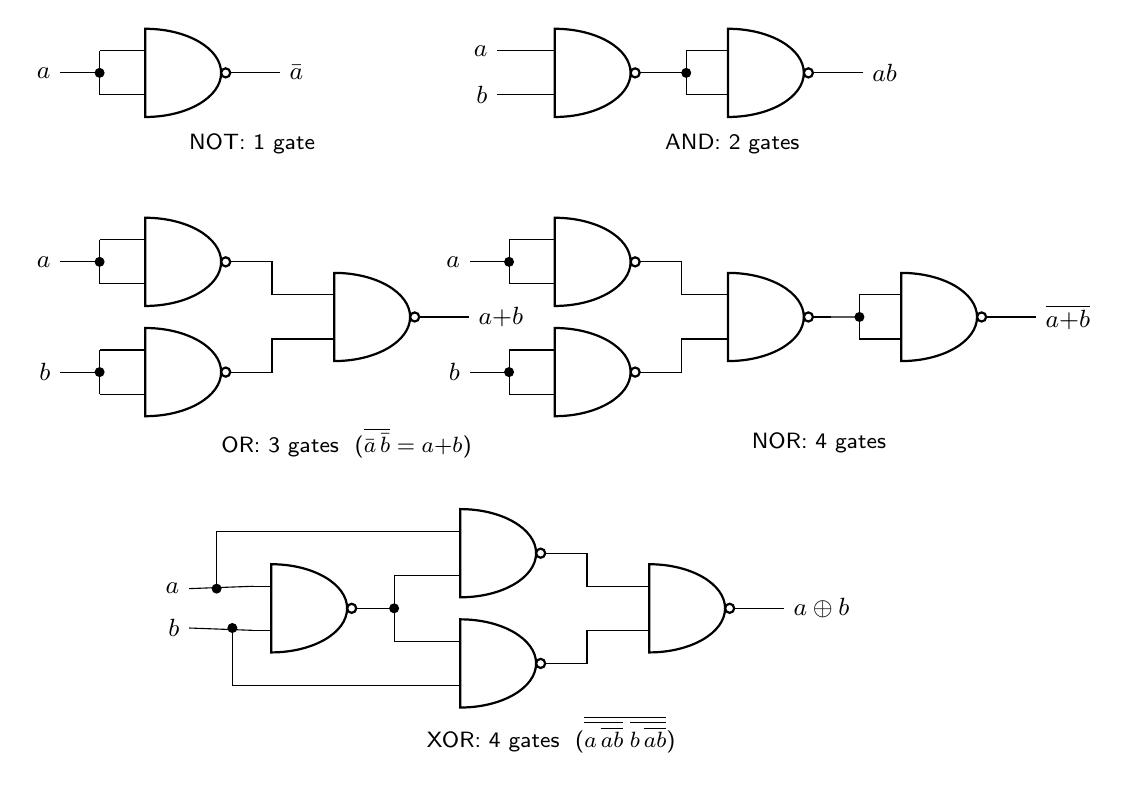
\begin{tikzpicture}[font=\sffamily\small]
  % ---- NOT: tie inputs ----
  \node[nand port] (not1) at (0,0) {};
  \draw (not1.in 1) -- ++(-0.35,0) coordinate (na);
  \draw (not1.in 2) -- ++(-0.35,0) coordinate (nb);
  \draw (na) -- (nb);
  \draw ($(na)!0.5!(nb)$) -- ++(-0.5,0) node[left]{$a$}; \node[circ] at ($(na)!0.5!(nb)$) {};
  \draw (not1.out) -- ++(0.4,0) node[right]{$\bar a$};
  \node[font=\sffamily\footnotesize] at (0.2,-0.9) {NOT: 1 gate};
  % ---- AND: NAND + NOT ----
  \node[nand port] (a1) at (5.2,0) {};
  \node[nand port] (a2) at (7.4,0) {};
  \draw (a1.in 1) -- ++(-0.5,0) node[left]{$a$};
  \draw (a1.in 2) -- ++(-0.5,0) node[left]{$b$};
  \draw (a2.in 1) -- ++(-0.3,0) coordinate (aa);
  \draw (a2.in 2) -- ++(-0.3,0) coordinate (ab);
  \draw (aa) -- (ab);
  \draw (a1.out) -- ($(aa)!0.5!(ab)$); \node[circ] at ($(aa)!0.5!(ab)$) {};
  \draw (a2.out) -- ++(0.4,0) node[right]{$ab$};
  \node[font=\sffamily\footnotesize] at (6.3,-0.9) {AND: 2 gates};
  % ---- OR: invert both inputs, then NAND ----
  \node[nand port] (o1) at (0,-2.4) {};
  \node[nand port] (o2) at (0,-3.8) {};
  \node[nand port] (o3) at (2.4,-3.1) {};
  \foreach \g/\l in {o1/a, o2/b}{
    \draw (\g.in 1) -- ++(-0.35,0) coordinate (\g a);
    \draw (\g.in 2) -- ++(-0.35,0) coordinate (\g b);
    \draw (\g a) -- (\g b);
    \draw ($(\g a)!0.5!(\g b)$) -- ++(-0.5,0) node[left]{$\l$}; \node[circ] at ($(\g a)!0.5!(\g b)$) {};}
  \draw (o1.out) -- ++(0.3,0) |- (o3.in 1);
  \draw (o2.out) -- ++(0.3,0) |- (o3.in 2);
  \draw (o3.out) -- ++(0.4,0) node[right]{$a{+}b$};
  \node[font=\sffamily\footnotesize] at (1.4,-4.7) {OR: 3 gates \ ($\overline{\bar a\,\bar b} = a{+}b$)};
  % ---- NOR: OR + NOT ----
  \node[nand port] (r1) at (5.2,-2.4) {};
  \node[nand port] (r2) at (5.2,-3.8) {};
  \node[nand port] (r3) at (7.4,-3.1) {};
  \node[nand port] (r4) at (9.6,-3.1) {};
  \foreach \g/\l in {r1/a, r2/b}{
    \draw (\g.in 1) -- ++(-0.35,0) coordinate (\g a);
    \draw (\g.in 2) -- ++(-0.35,0) coordinate (\g b);
    \draw (\g a) -- (\g b);
    \draw ($(\g a)!0.5!(\g b)$) -- ++(-0.5,0) node[left]{$\l$}; \node[circ] at ($(\g a)!0.5!(\g b)$) {};}
  \draw (r1.out) -- ++(0.3,0) |- (r3.in 1);
  \draw (r2.out) -- ++(0.3,0) |- (r3.in 2);
  \draw (r4.in 1) -- ++(-0.3,0) coordinate (ra);
  \draw (r4.in 2) -- ++(-0.3,0) coordinate (rb);
  \draw (ra) -- (rb);
  \draw (r3.out) -- ($(ra)!0.5!(rb)$); \node[circ] at ($(ra)!0.5!(rb)$) {};
  \draw (r4.out) -- ++(0.4,0) node[right]{$\overline{a{+}b}$};
  \node[font=\sffamily\footnotesize] at (7.4,-4.7) {NOR: 4 gates};
  % ---- XOR: classic 4-NAND ----
  \node[nand port] (x1) at (1.6,-6.8) {};
  \node[nand port] (x2) at (4.0,-6.1) {};
  \node[nand port] (x3) at (4.0,-7.5) {};
  \node[nand port] (x4) at (6.4,-6.8) {};
  \coordinate (xa) at (-0.6,-6.55);
  \coordinate (xb) at (-0.6,-7.05);
  \draw (xa) node[left]{$a$} -- (x1.in 1);
  \draw (xb) node[left]{$b$} -- (x1.in 2);
  \draw ($(xa)+(0.35,0)$) |- (x2.in 1); \node[circ] at ($(xa)+(0.35,0)$) {};
  \draw ($(xb)+(0.55,0)$) |- (x3.in 2); \node[circ] at ($(xb)+(0.55,0)$) {};
  \draw (x1.out) -- ++(0.25,0) coordinate (xm);
  \draw (xm) |- (x2.in 2);
  \draw (xm) |- (x3.in 1); \node[circ] at (xm) {};
  \draw (x2.out) -- ++(0.3,0) |- (x4.in 1);
  \draw (x3.out) -- ++(0.3,0) |- (x4.in 2);
  \draw (x4.out) -- ++(0.4,0) node[right]{$a \oplus b$};
  \node[font=\sffamily\footnotesize] at (4.0,-8.4) {XOR: 4 gates \ ($\overline{\overline{a\,\overline{ab}}\;\overline{b\,\overline{ab}}}$)};
\end{tikzpicture}
\end{document}
